%%%%%%%%%%%%%%%%%%%%%%%%%%%%%%%%%%%%%%%%%
% a0poster Landscape Poster
% LaTeX Template
% Version 1.0 (22/06/13)
%
% The a0poster class was created by:
% Gerlinde Kettl and Matthias Weiser (tex@kettl.de)
% 
% This template has been downloaded from:
% http://www.LaTeXTemplates.com
%
% License:
% CC BY-NC-SA 3.0 (http://creativecommons.org/licenses/by-nc-sa/3.0/)
%
%%%%%%%%%%%%%%%%%%%%%%%%%%%%%%%%%%%%%%%%%

%----------------------------------------------------------------------------------------
%	PACKAGES AND OTHER DOCUMENT CONFIGURATIONS
%----------------------------------------------------------------------------------------

\documentclass[a0,landscape]{a0poster}

\usepackage{multicol} % This is so we can have multiple columns of text side-by-side
\columnsep=100pt % This is the amount of white space between the columns in the poster
\columnseprule=3pt % This is the thickness of the black line between the columns in the poster

\usepackage[svgnames]{xcolor} % Specify colors by their 'svgnames', for a full list of all colors available see here: http://www.latextemplates.com/svgnames-colors

\usepackage{times} % Use the times font
%\usepackage{palatino} % Uncomment to use the Palatino font

\usepackage{graphicx} % Required for including images
\graphicspath{{figures/}} % Location of the graphics files
\usepackage{booktabs} % Top and bottom rules for table
\usepackage[font=small,labelfont=bf]{caption} % Required for specifying captions to tables and figures
\usepackage{amsfonts, amsmath, amsthm, amssymb} % For math fonts, symbols and environments
\usepackage{wrapfig} % Allows wrapping text around tables and figures
 \usepackage{float}
 \usepackage{hyperref}
\begin{document}

%----------------------------------------------------------------------------------------
%	POSTER HEADER 
%----------------------------------------------------------------------------------------

% The header is divided into three boxes:
% The first is 55% wide and houses the title, subtitle, names and university/organization
% The second is 25% wide and houses contact information
% The third is 19% wide and houses a logo for your university/organization or a photo of you
% The widths of these boxes can be easily edited to accommodate your content as you see fit

\begin{minipage}[b]{0.55\linewidth}
\veryHuge \color{NavyBlue} \textbf{Honeypot Configuration and Data Analysis} \color{Black}\\ % Title
%\Huge\textit{Honeypot Configuration and Data Analysis}\\[1cm] % Subtitle
\huge \textbf{Jared Campbell \& David Zehden}\\ % Author(s)
\huge The University of Texas at Austin\\ % University/organization
\end{minipage}
%
%
%
\begin{minipage}[b]{0.19\linewidth}
%
\includegraphics[width=20cm]{logo.png} % Logo or a photo of you, adjust its dimensions here
\end{minipage}

\vspace{1cm} % A bit of extra whitespace between the header and poster content

%----------------------------------------------------------------------------------------

\begin{multicols}{3} % This is how many columns your poster will be broken into, a poster with many figures may benefit from less columns whereas a text-heavy poster benefits from more

%----------------------------------------------------------------------------------------
%	ABSTRACT
%----------------------------------------------------------------------------------------

\color{Black} % Navy color for the abstract

%\begin{figure}[H]
%	\begin{center}
%	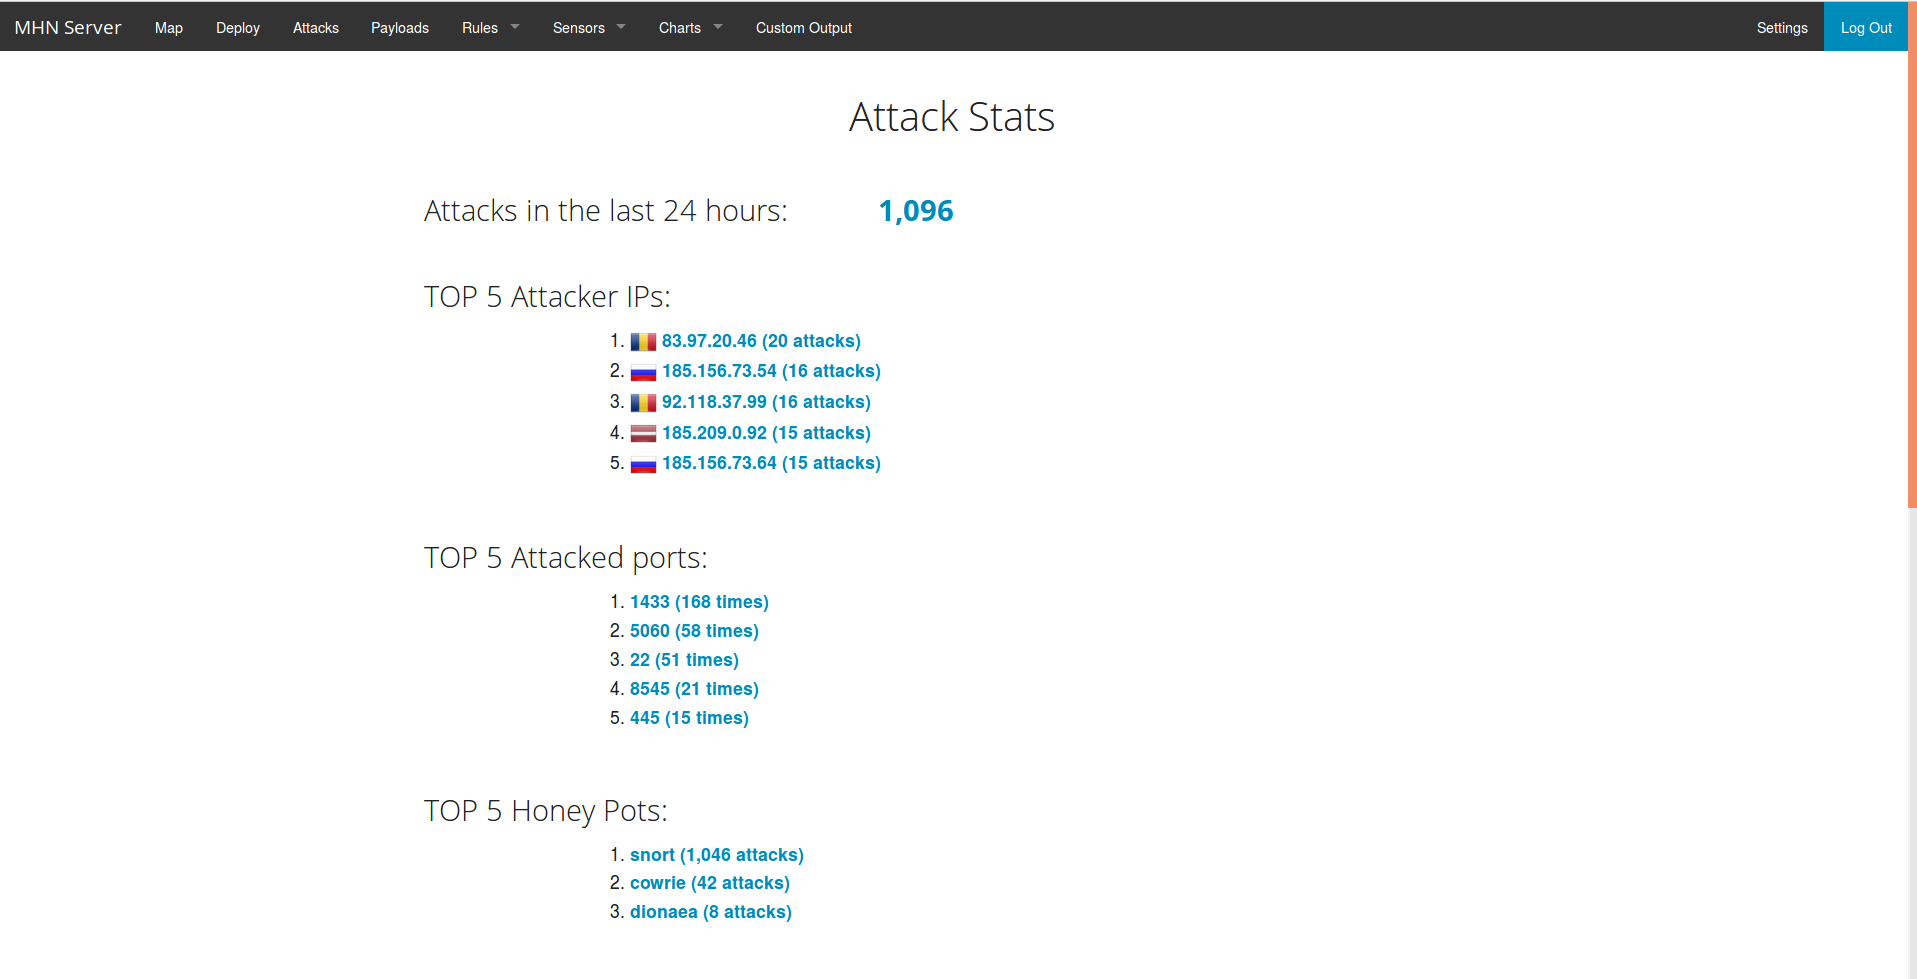
\includegraphics[width=30cm]{mhn.png}
%	\caption{The Modern Honeypot Network Dashboard}
%	\end{center}
%\end{figure} 
%\begin{center}[H]
%	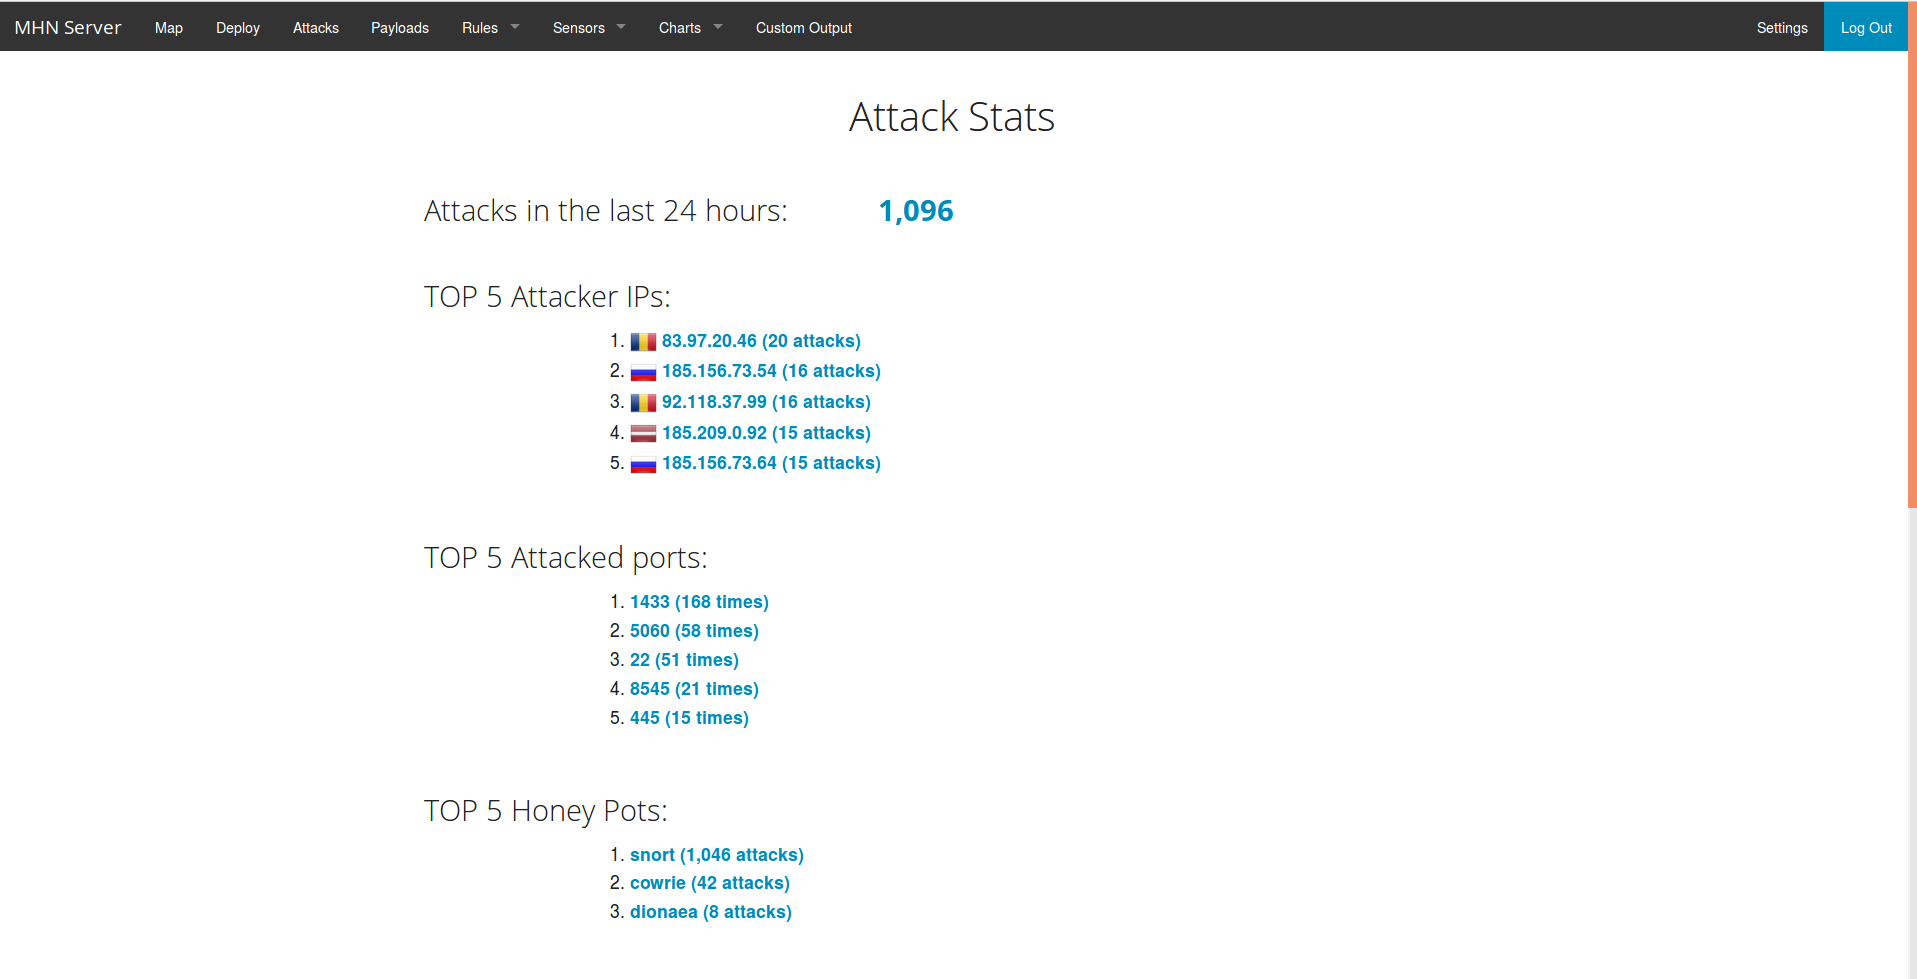
\includegraphics[width=20cm]{mhn.png} % Logo or a photo of you, adjust its dimensions here
	
%\end{center}
%----------------------------------------------------------------------------------------
%	OBJECTIVES
%----------------------------------------------------------------------------------------

\color{Black} % DarkSlateGray color for the rest of the content

\section*{Main Objectives}

\begin{enumerate}
\item Setup Amazon Web Services EC2 instance
\item Explore Honeypot options
\item Deploy Honeypot of choice on AWS
\item Configure Honeypot as needed
\item Collect data over time
\item Explore collected data to determine trends
\end{enumerate}

%----------------------------------------------------------------------------------------
%	MATERIALS AND METHODS
%----------------------------------------------------------------------------------------

\section*{Results}
Our honeypot made over 20,000 detections. We received traffic from all over the world, as you can see in Figure 2. In order to generate this map, we took all the IPs we detected and used the \href{https://github.com/pieqq/PyGeoIpMap}{PyGeoIpMap} library.
\begin{figure}[H]
	\begin{center}
		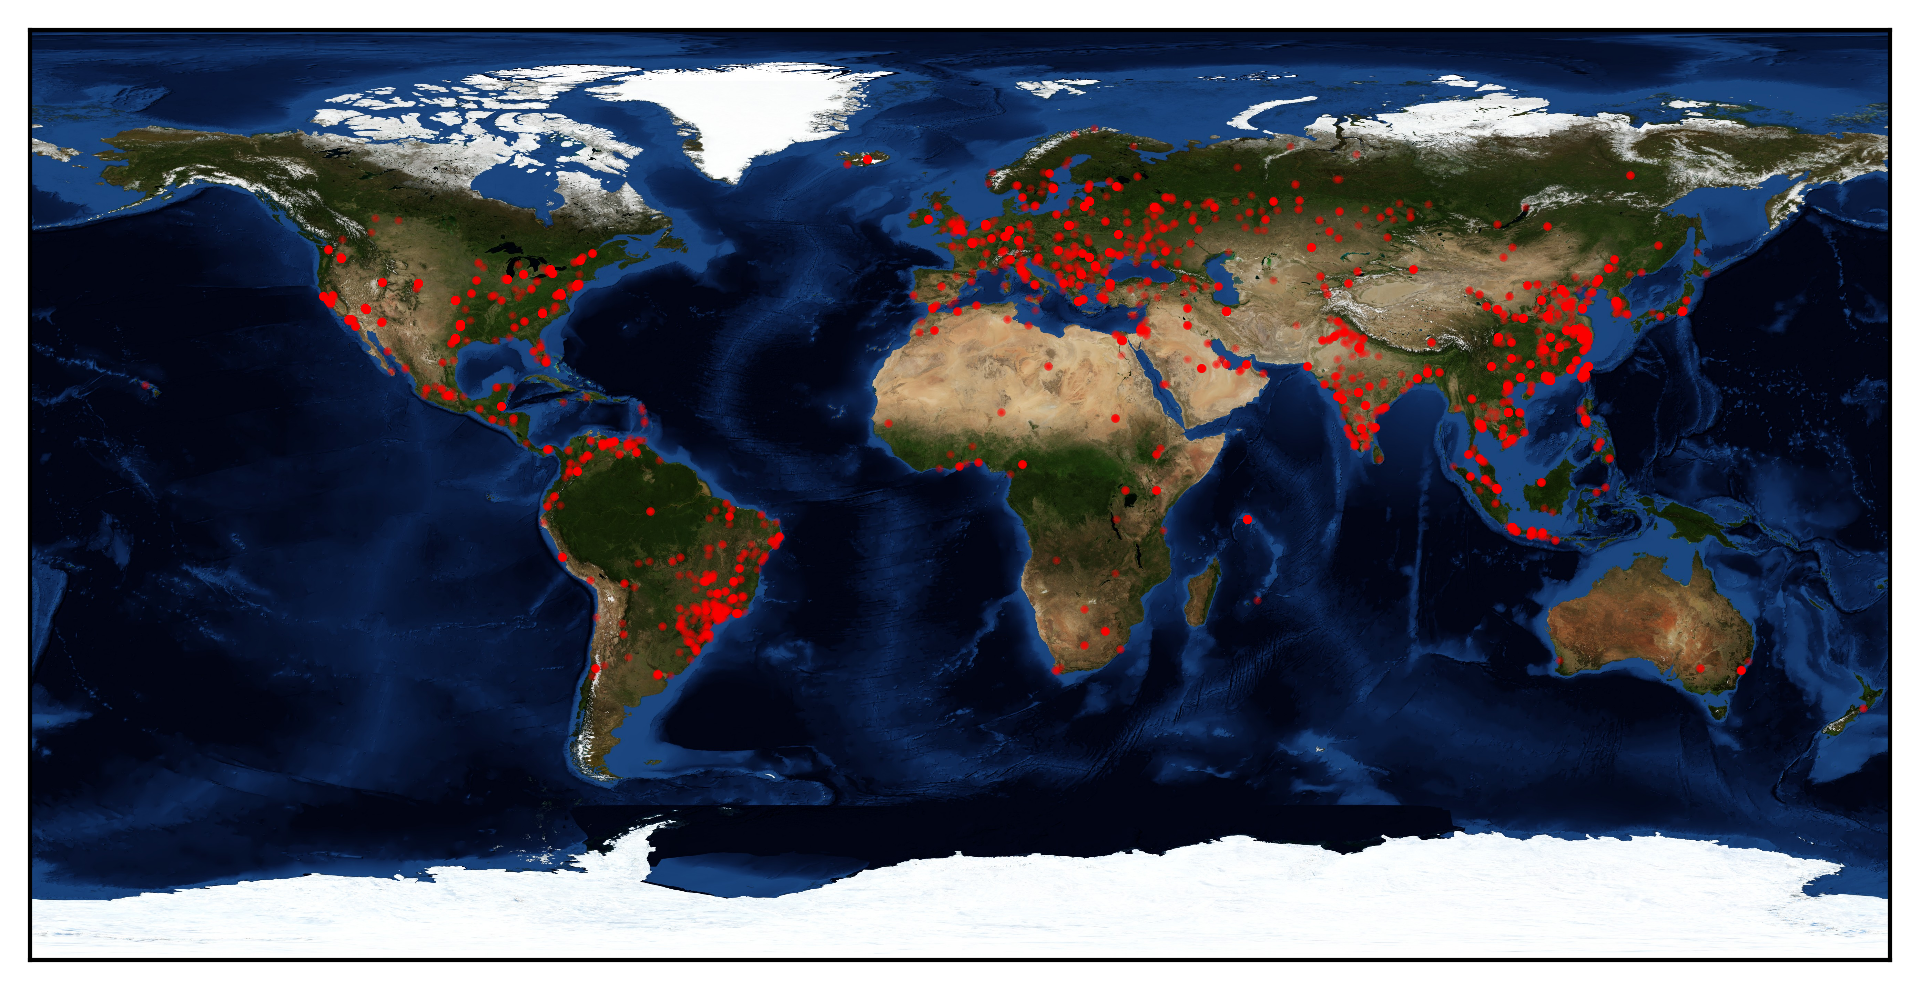
\includegraphics[width=30cm]{map.png}
		\caption{Approximate Locations of Detected IP Addresses}
	\end{center}
\end{figure} 

\begin{figure}[H]
	\begin{center}
		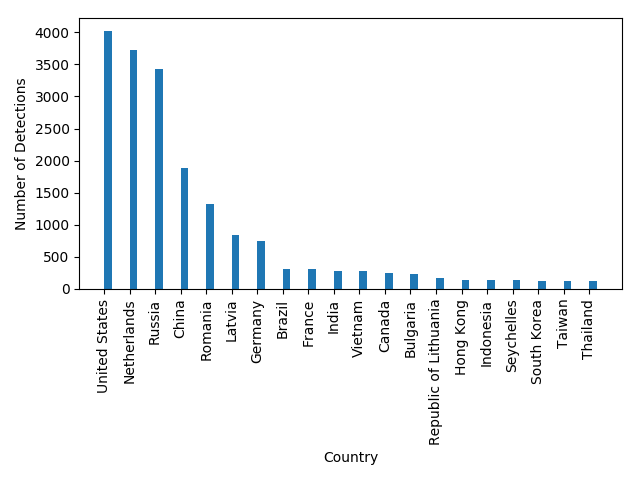
\includegraphics[width=25cm]{top_countries.png}
		\caption{Breakdown of Detections by Country}
	\end{center}
\end{figure} 

\begin{figure}[H]
	\begin{center}
		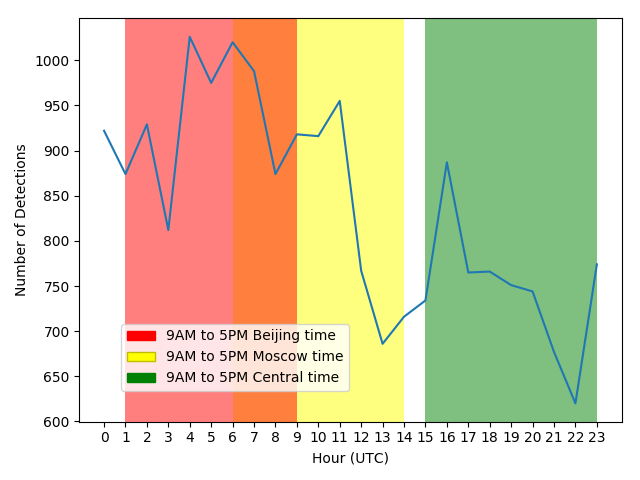
\includegraphics[width=20cm]{time_breakdown.png}
		\caption{Breakdown of Detections by Time of Day (UTC)}
	\end{center}
\end{figure} 

\begin{figure}[H]
	\begin{center}
		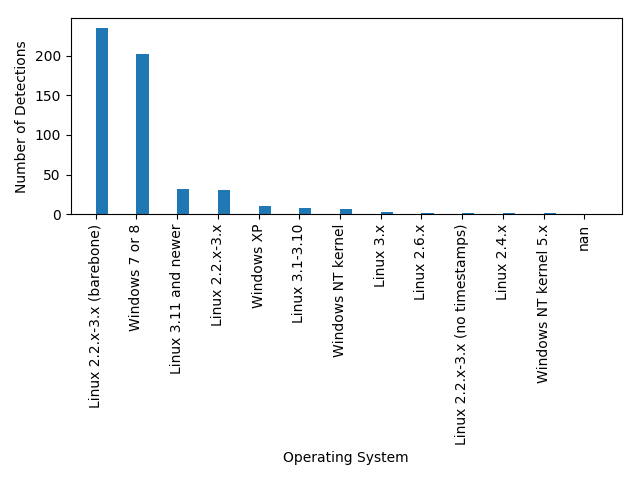
\includegraphics[width=25cm]{top_os.png}
		\caption{Breakdown of Detected Operating Systems}
	\end{center}
\end{figure} 

\begin{figure}[H]
	\begin{center}
		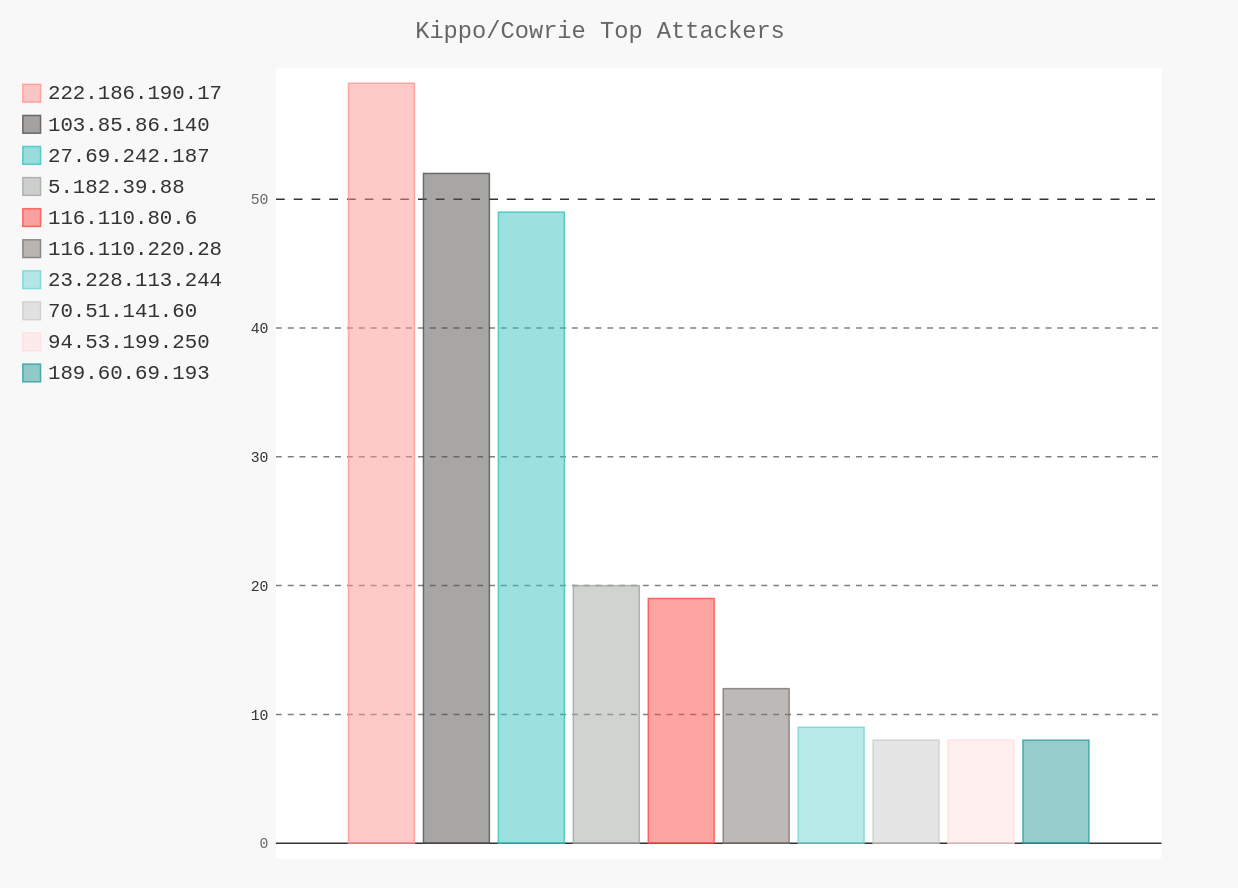
\includegraphics[width=20cm]{images/top_attackers.png}
		\caption{IP Addresses of Top Attackers}
	\end{center}
\end{figure} 

\begin{figure}[H]
	\begin{center}
		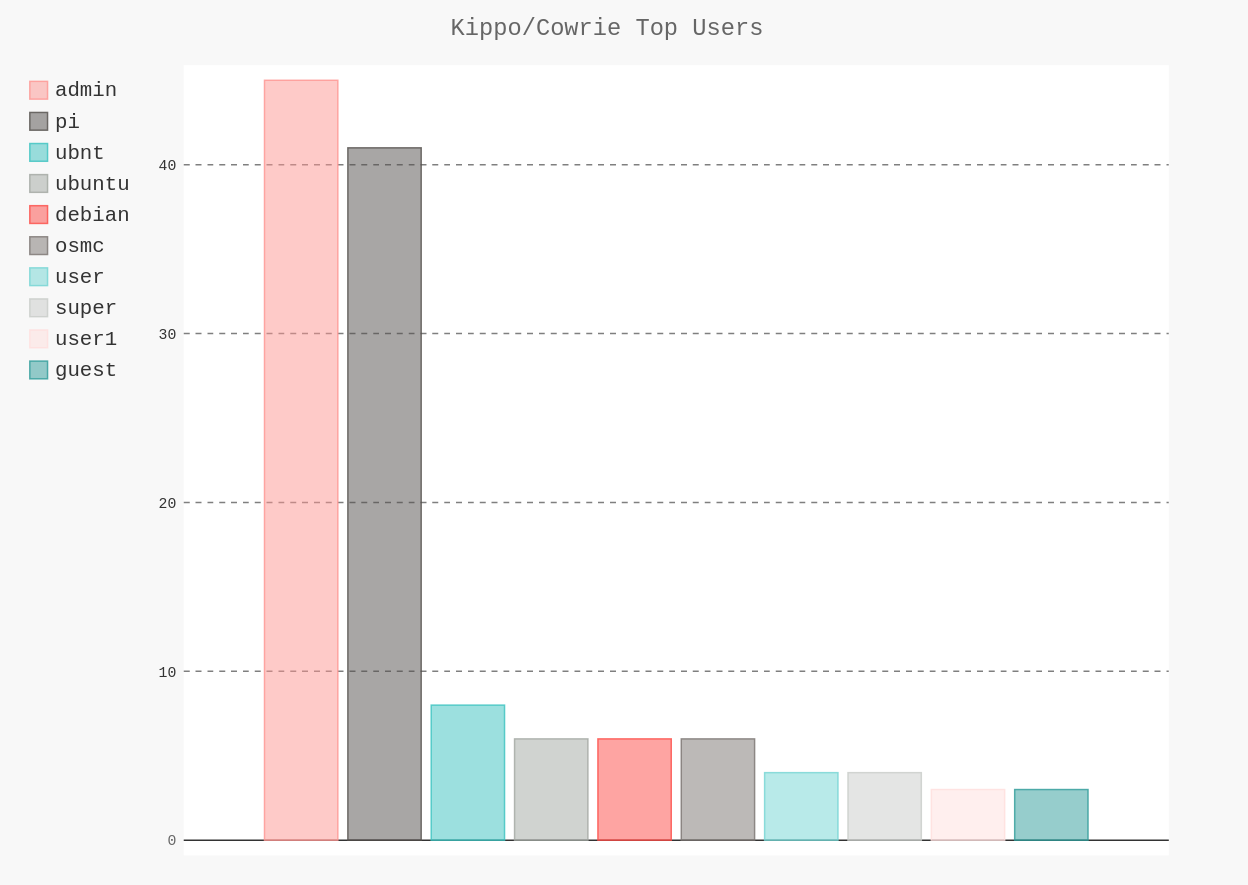
\includegraphics[width=20cm]{images/top_users.png}
		\caption{Top Usernames Attempted}
	\end{center}
\end{figure}

\begin{figure}[H]
	\begin{center}
		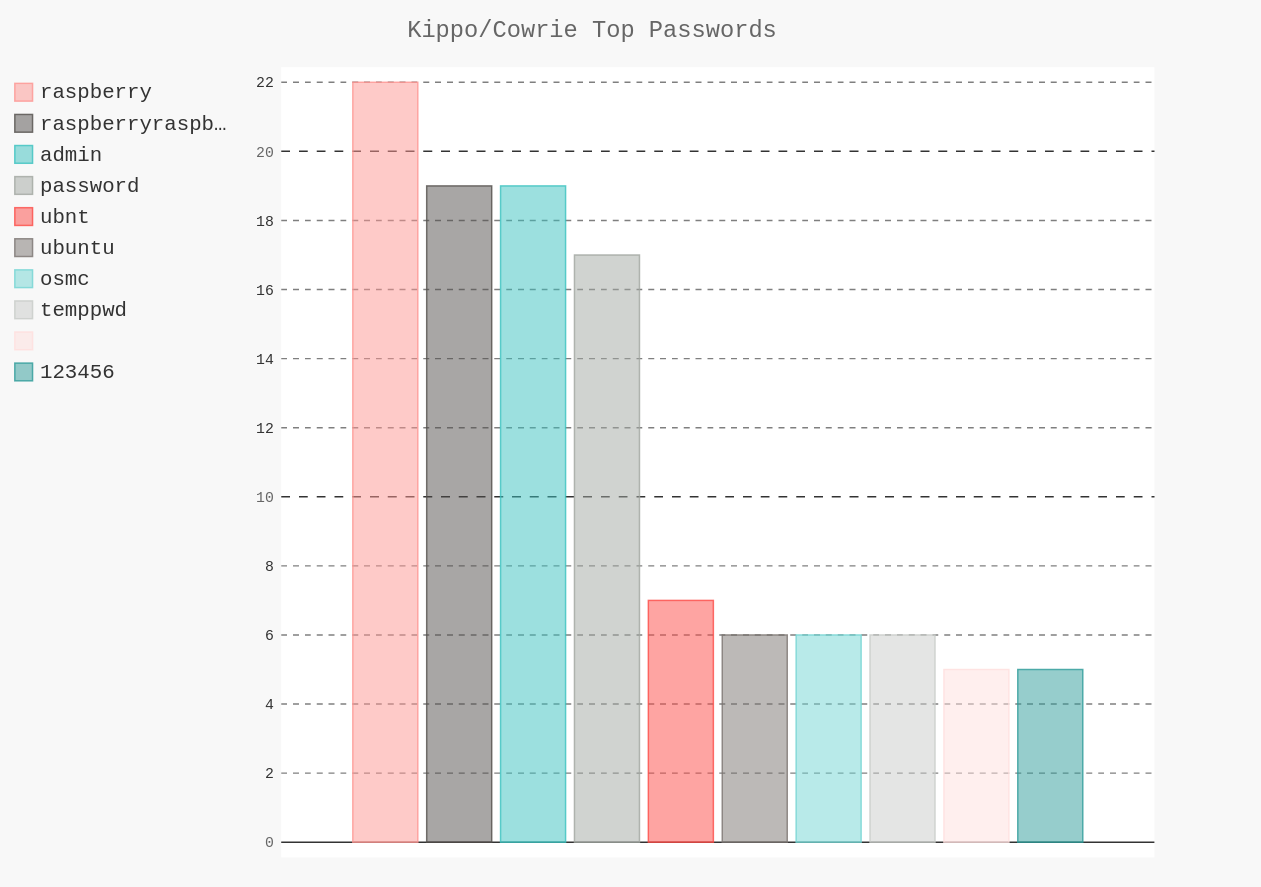
\includegraphics[width=20cm]{images/top_pass.png}
		\caption{Top Passwords Attempted}
	\end{center}
\end{figure}


%------------------------------------------------
%----------------------------------------------------------------------------------------
%	RESULTS 
%----------------------------------------------------------------------------------------

\section*{Honeypot Use Cases}
\begin{itemize}
	\item Defending an Enterprise Network
	\begin{itemize}
		\item Analyze trends in attacks against an organization's network
		\item Slow down attackers by allowing them to target a honeypot instead of critical infrastructure
	\end{itemize}
		\item Information Security Research
	\begin{itemize}
		\item Gather data on attack trends across the internet
		\item Discover potential zero-day attacks
	\end{itemize}
\end{itemize}

%----------------------------------------------------------------------------------------

\end{multicols}
\end{document}
